\documentclass{beamer}
\mode <presentation>
{
    \usetheme{boxes}
    \usecolortheme{crane}
    \setbeamercovered{transparent}
}

\usepackage[absolute,overlay]{textpos}
\usepackage{pgf,pgfarrows,pgfnodes}
\usepackage[english]{babel}
\usepackage{lmodern}
\usepackage{newcent}
\usepackage{amsmath}
\usepackage{listings}
% math extension - one probably wants to use symbols like '[' (written as '$[$')
\usepackage{ucs}
%\usepackage[utf8]{inputenc}
%\usefonttheme{structuresmallcapsserif}

% utf8x does not work with xetex
\usepackage[utf8x]{inputenc}

\usepackage[normalem]{ulem}


\setlength{\TPHorizModule}{1mm}
\setlength{\TPVertModule}{1mm}
\newcommand{\WorkInProgress}{%
\begin{textblock}{14}(120.0,75.7)

\includegraphics[height=0.1cm]{./pics/logo_owf.png}
\end{textblock}
  }

%\setbeamercolor{background canvas}{bg=\includegraphics[width=\textwidth]{./pics/wolf.png}}

\title{FusionInventory}
\author{{FusionInventory.org}}
\subject{Assets management with FusionInventory and GLPI}
\keywords{Assets management, Inventory, FusionInventory, GLPI}

\date{Juin 2012}
%\titlegraphic{GLPI}
%subtitle{\includegraphics[width=1.2cm]{./pics/fusioninventory-logo.png}}
\institute{
\includegraphics[height=1.2cm]{./pics/mongueur.png}}

\titlegraphic{}
\subtitle{Journées Perl}
\institute{Strasbourg}
\author{ Gonéri Le Bouder \texttt{<goneri@teclib.com>}}
\logo{\includegraphics[height=0.7cm]{./pics/fusioninventory-logo.pdf}}

\AtBeginSection[] % Do nothing for \section*
{
    \begin{frame}<beamer>
        \frametitle{Outline}
        \tableofcontents[currentsection]
    \end{frame}
}

%%%%%%%%%%%%%%%%%%%%%%%%%%%%%%%%%%%%%%%%%%%%%%%
%%%%%%%%%%%%%%%%%%%%%%%%%%%%%%%%%%%%%%%%%%%%%%%
\begin{document}

\frame[plain]{\titlepage}


\begin{frame}
    \frametitle{A propos de moi}


    \begin{block}{Gonéri Le Bouder}
        \begin{itemize}
        \item Développeur FusionInventory
        \item Développeur Debian
        \item Mongueur Perl
        \item Travaille chez TECLIB', Paris
        \end{itemize}
    \end{block}

\end{frame}

\section{Vue d'ensemble}

\begin{frame}
    \frametitle{Les origines du logiciel}

    \begin{description}
      \item[2006] Création de l'agent
      \item[2008] Début du serveur (le plugin GLPI, Tracker)
      \item[2009] Intégration Agent/Serveur
      \item[2010] Projet FusionInventory
      \item[2010] Intégration avec Uranos
      \item[2011] Intégration avec Rudder (cfengine)
      \item[2012] Intégration avec OTRS
    \end{description}

\end{frame}



\begin{frame}
    \frametitle{La structure du projet}
    %%-------------------------------------------------------------------
    %%\logo{\includegraphics[height=3.5cm]{./pics/glpi-doc.png}}
    FusionInventory est un projet communautaire.

    \begin{itemize}
        \item liste de diffusion active
        \item IRC: \#FusionInventory sur FreeNode
        \item Forge, dépôt Git, etc
    \end{itemize}
\end{frame}


\begin{frame}
    \frametitle{Les contributeurs}

 \begin{columns}
 \begin{column}[T]{4cm}
    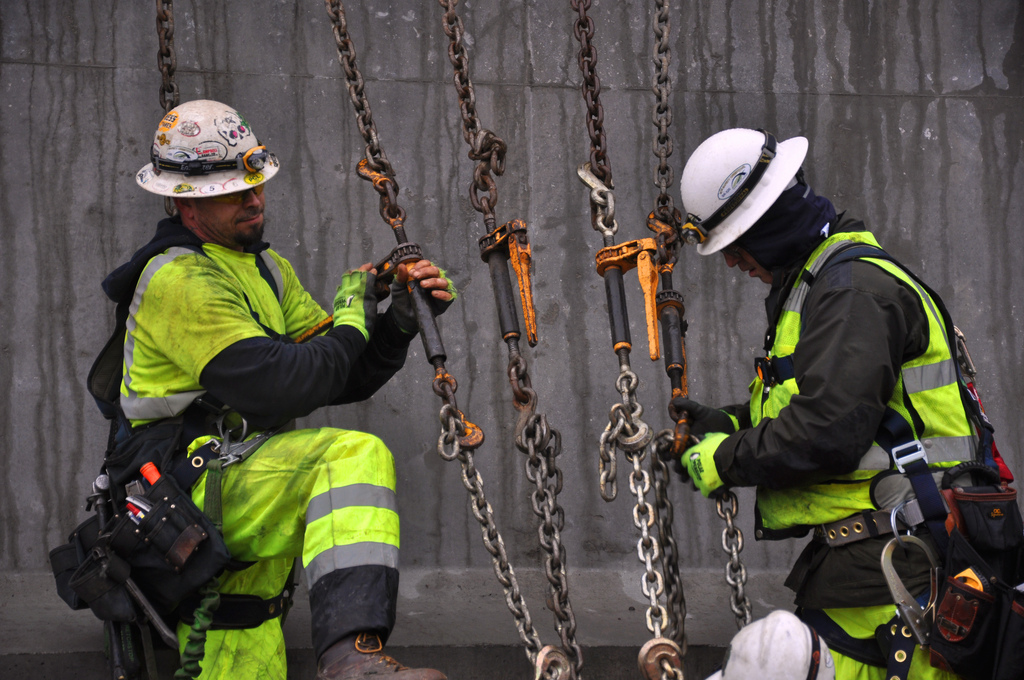
\includegraphics[height=3.7cm]{./pics/worker.jpg}
 \end{column}
 \begin{column}[t]{5cm}
    \begin{itemize}
    \item 4 développeurs réguliers
    \item une communauté active
    \item 2 entreprises parties prenantes
    \end{itemize}

 \end{column}
\end{columns}

    \pause
    \bf{Nous aimons le sang chaud !}
\end{frame}



\begin{frame}
    \frametitle{Un peu de vocabulaire}

    \begin{block}{FusionInventory n'est pas directement un logiciel}
    \begin{itemize}
        \item Agent: un logiciel destiné aux machines du parc
        \item Serveur: dialogue avec le serveur
        \item Tâche: une actione effectuée par un agent pour le serveur
    \end{itemize}
    \end{block}

\end{frame}


\begin{frame}
    \frametitle{Les serveurs aujourd'hui}

    \begin{block}{4 solutions aujourd'hui}
        \begin{itemize}
            \item FusionInventory for GLPI \\
            \url{http://www.FusionInventory.org}
            \item Uranos \\
            \url{http://uranos.sourceforge.net/}
            \item Rudder de Normation \\
            \url{http://www.normation.com/\#produits}
            \item OCS Inventory NG
            \item Pulse 2 de Mandriva

        \end{itemize}
        ... il est aussi possible de produire un inventaire XML en local.
    \end{block}

\end{frame}

\begin{frame}
    \frametitle{Des intégrations sont en discution avec}

    \begin{itemize}
    \item FusionDirectory
    \item OTRS ITSM (développement pratiquement terminé)
    \end{itemize}
\end{frame}

\begin{frame}
    \frametitle{pull / push}

    \begin{block}{FusionInventory permet le "push" ou "pull"}
    \begin{itemize}
    \item \textbf{"pull": Agent $\Longrightarrow$ Serveur} \\
    l'agent est à l'origine du dialogue.
    \item \textbf{"push": Agent $\Longleftarrow$ Serveur} \\
    le serveur commence le dialogue.
    \end{itemize}
    \end{block}

\end{frame}

\begin{frame}
    \frametitle{Agent: Installation}


    \begin{block}{different options}
        \begin{itemize}
            \item \textbf{distribution packages} \\
            \small{Debian, Fedora, EPEL, Ubuntu, Mageia, ...}
            \item \textbf{Windows installer} \\
            \small{GPO, psexec, ...}
            \item \textbf{static prebuilt packages}, untar and run \\
            \small{62 differents system so far}
            \item tarball or CPAN installation
        \end{itemize}
    \end{block}
\end{frame}

\begin{frame}
    \frametitle{Agent: Installation}

   \begin{columns}
   \begin{column}{0.35\textwidth}

\includegraphics[height=5.5cm]{pics/googleplay.png}
 \end{column}
 \begin{column}{0.65\textwidth}
Sur Androïd, l'application est sur Google Play.
 \end{column}
\end{columns}

\end{frame}


\section{Agent : OS supporté}

\begin{frame}
    \frametitle{Les systèmes d'exploitation supportés}

    \begin{itemize}
        \item Linux
        \item Windows, depuis 2000
        \item MacOSX 
        \item BSD
        \item AIX
        \item HP-UX
        \item Solaris
        \item Android
    \end{itemize}


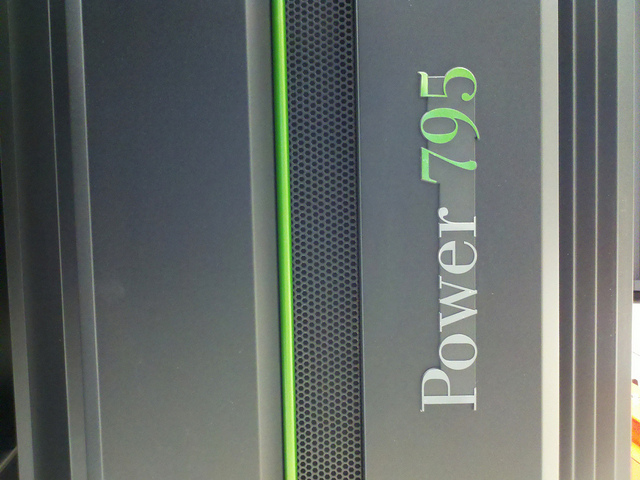
\includegraphics[height=0.5cm]{pics/logos/aix.png}
\includegraphics[height=0.5cm]{pics/logos/fedora.png}
\includegraphics[height=0.5cm]{pics/logos/hp-ux.png}
\includegraphics[height=0.5cm]{pics/logos/netbsd.png}
\includegraphics[height=0.5cm]{pics/logos/openbsd.png}

\includegraphics[height=0.5cm]{pics/logos/solaris.jpg}
\includegraphics[height=0.5cm]{pics/logos/centos.jpg}

\includegraphics[height=0.5cm]{pics/logos/linux.png}
\includegraphics[height=0.5cm]{pics/logos/osx.png}
\includegraphics[height=0.5cm]{pics/logos/ubuntu.png}
\includegraphics[height=0.5cm]{pics/logos/debian.png}
\includegraphics[height=0.5cm]{pics/logos/freebsd.png}
\includegraphics[height=0.5cm]{pics/logos/redhat.png}
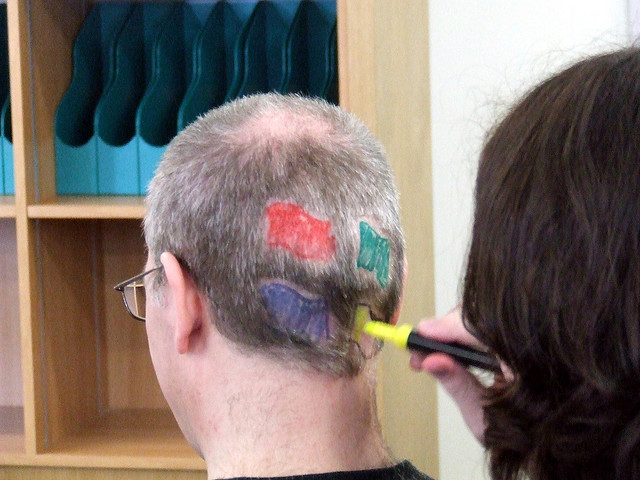
\includegraphics[height=0.5cm]{pics/logos/windows.jpg}
\includegraphics[height=0.5cm]{pics/logos/dragonflybsd.png}
\includegraphics[height=0.5cm]{pics/logos/mageia.png}

\end{frame}

\begin{frame}    
    \begin{block}{Perl aide beaucoup}
        \begin{itemize}
            \item Peu de différences fondamentales en les UNIX like
            \item Il reste Win32
        \end{itemize}
    \end{block}
\end{frame}

\section{Tâche : Découverte du réseau}

\begin{frame}
    \frametitle{Découverte du réseau}

    \begin{block}{Une remontée rapide des éléments actifs}
    \begin{itemize}
      \item NMAP 
      \item NetBios
      \item requête SNMP
    \end{itemize}
    \end{block}

\end{frame}

\section{Tâche : Inventaire réseau}
%\begin{frame}
%    \frametitle{Remote SNMP inventory}
%
%    \begin{block}{Network devices}
%        \begin{itemize}
%            \item serial number, firmware, ...
%            \item ports mapping
%        \end{itemize}
%    \end{block}
%
%    \begin{block}{Network printers}
%        \begin{itemize}
%            \item serial number, firmware, ...
%            \item cartridge ink level
%            \item page counter
%        \end{itemize}
%    \end{block}
%\end{frame}

\begin{frame}
    \frametitle{... INTERM\`{E}DE ...}

%   \begin{columns}
%   \begin{column}{0.35\textwidth}
         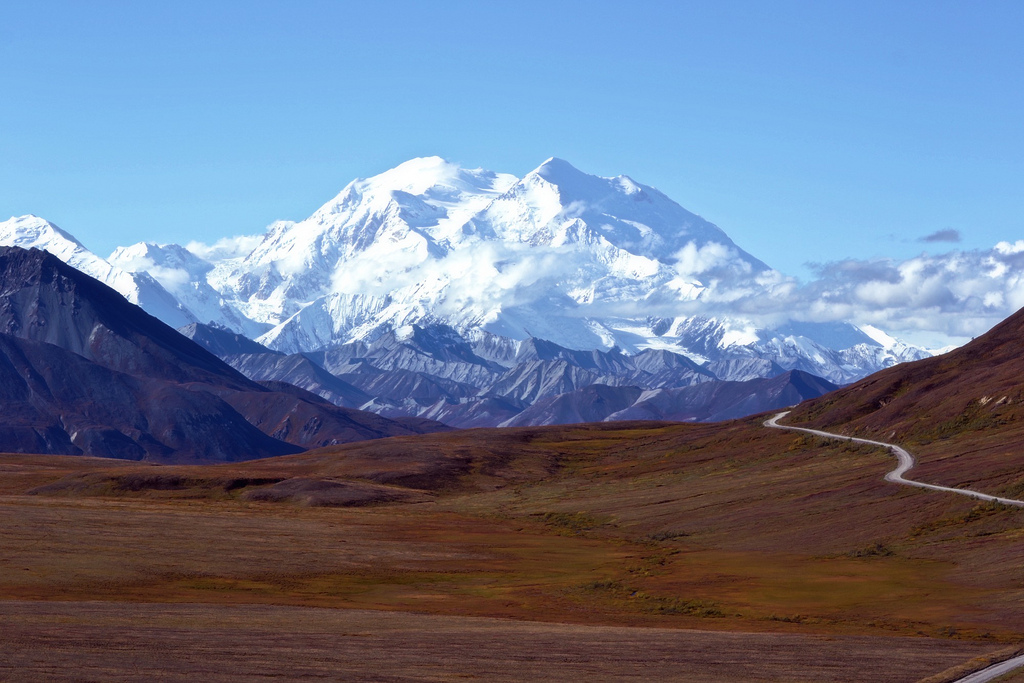
\includegraphics[height=7.5cm]{./pics/montagne.jpg}
% \end{column}
% \begin{column}{0.65\textwidth}
%    \begin{block}{... INTERM\`{E}DE ...}
%    \end{block}

% \end{column}
%\end{columns}
\end{frame}


\begin{frame}
    \frametitle{SNMP}

%    \begin{center}
%    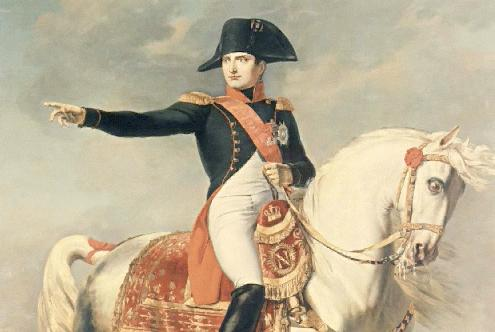
\includegraphics[height=4.0cm]{pics/napoleon.jpg}
%    \end{center}

    \begin{block}{L'origine de SNMP}
    \begin{itemize}
    \item Un standard \\
    \small{Première RFC: 1988}
    \item Créé pour superviser les équipements
    \item 3 versions différentes 1, 2c, 3 (Chiffrement)
    \item OID: L'adresse d'une information
    \item MIB: Un catalogue d'OID
    \end{itemize}
    \end{block}
\end{frame}

\begin{frame}
    \frametitle{SNMP: Pour faire quoi?}

    \begin{block}{Quelle utilisation de SNMP?}
    \begin{itemize}
    \item Identifier les équipements distants (commutateurs, imprimantes, ...)
    \item Faire un inventaire
    \item Collecter les informations importantes
    \end{itemize}
    \end{block}
\end{frame}

\begin{frame}
    \frametitle{SNMP: Le cauchemar}

    \begin{block}{“Vous pouvez supporter mon équipement, j'ai la MIB !”}

    \pause
    \begin{itemize}
    \item En règle générale, elles sont dures à trouver
    \item Rarement libres ou pire, redistribuable
    \item Des informations importantes sont souvant absentes
    \item Le pire ! Elles sont bien souvant fausse !
    \end{itemize}
    \end{block}

%    \begin{block}{With our SNMP models, we are sure device is well supported!}
%    \end{block}
\end{frame}
\begin{frame}
    \frametitle{SNMP: Un exemple}

 \begin{columns}
 \begin{column}{0.35\textwidth}
         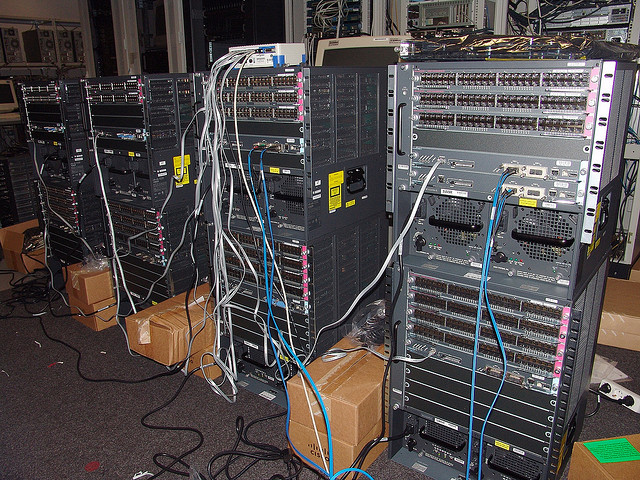
\includegraphics[height=7.5cm]{./pics/cisco.jpg}
 \end{column}
 \begin{column}{0.65\textwidth}
    \begin{block}{Exemple: Cisco 6500 firmware}
    12.2(33)SXI\textbf{2a} (02-Sep-09 01:00)
    \begin{itemize}
    \item Serial OID: .1.3.6.1.2.1.47.1.1.1.1.11.\textbf{1}
    \end{itemize}
    12.2(33)SXI\textbf{3} (27-Oct-09 11:12)
    \begin{itemize}
    \item Serial OID: .1.3.6.1.2.1.47.1.1.1.1.11.\textbf{2}$\Longleftarrow$ Gni?!
    \end{itemize}
    \end{block}

 \end{column}
\end{columns}


    
\end{frame}

\begin{frame}
    \frametitle{SNMP: aïe}

 \begin{columns}
 \begin{column}{0.35\textwidth}
         
\includegraphics[height=7.5cm]{./pics/dead-teletubbies.jpg}
 \end{column}
 \begin{column}{0.65\textwidth}

 \end{column}
\end{columns}
\end{frame}



\begin{frame}
    \frametitle{SNMP: Comment être fiable?}

    \begin{block}{On prépare nos propres “MIB”}
    \begin{itemize}
    \item Un travail manuel pour chaque équipement
    \item Des fichiers XML
    \item Définition des relations entre les OID et les infos \\
        \small{ex: numéro de série → OID 1.2.4.34.53...}
    \item Support des OID dynamiques
    \end{itemize}
    \end{block}


\end{frame}

\begin{frame}
    \frametitle{... FIN DE L'INTERM\`{E}DE ...}

    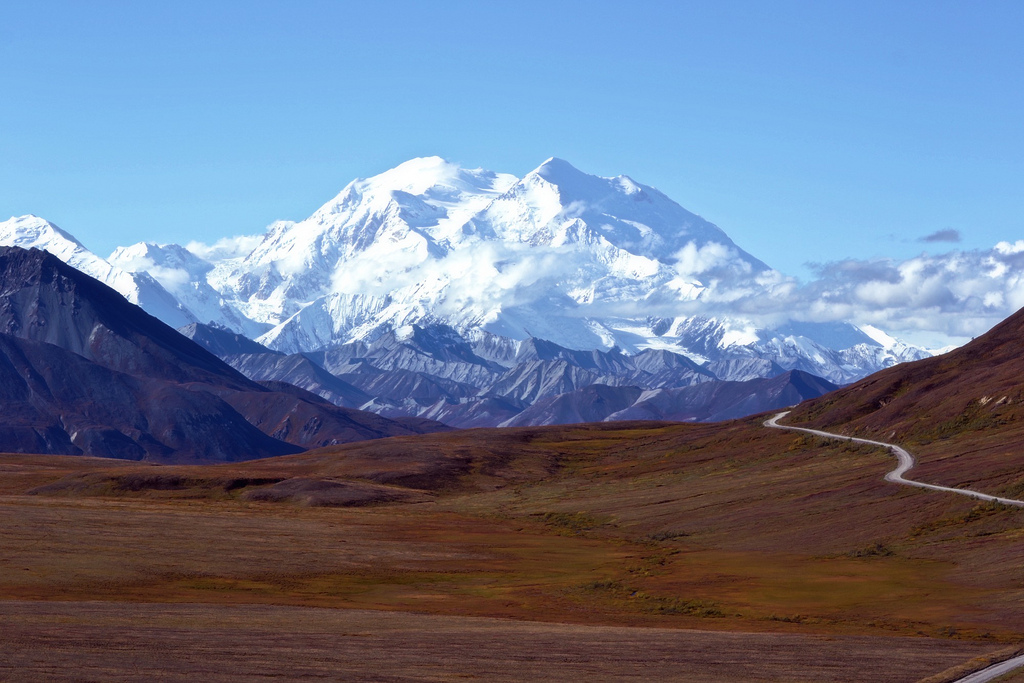
\includegraphics[height=7.5cm]{./pics/montagne.jpg}

\end{frame}



\begin{frame}
    \frametitle{SNMP: Commutateur (1/3)}

    \begin{block}{Informations générales}
    \begin{itemize}
    \item Numéro de série
    \item Fabriquant
    \item Modèle
    \item Version du firmware
    \item Adresse MAC
    \item Charge CPU / RAM
    \item etc
    \end{itemize}
    \end{block}
\end{frame}

\begin{frame}
    \frametitle{SNMP: Commutateur (2/3)}

    \begin{block}{Informations spécifiques (support avancé)}
    \begin{itemize}
    \item Nom des ports 
    \item La vitesse
    \item Le statut
    \item Les compteurs d'erreurs
    \item VLAN
    \item Trunk (taggé)
    \item ...
    \end{itemize}
    \end{block}
\end{frame}

\begin{frame}
    \frametitle{SNMP: Commutateur (3/3)}

    \begin{block}{Connexion par port}
    \begin{itemize}
    \item Adresse MAC \\ 
    \small{une à “n”}
    \item Découverte LLDP / CDP (Cisco) \\
    \small{remontée POIP}
    \end{itemize}
    \end{block}
\end{frame}

\begin{frame}
    \frametitle{SNMP: exemple d'un commutateur}

    \begin{center}
    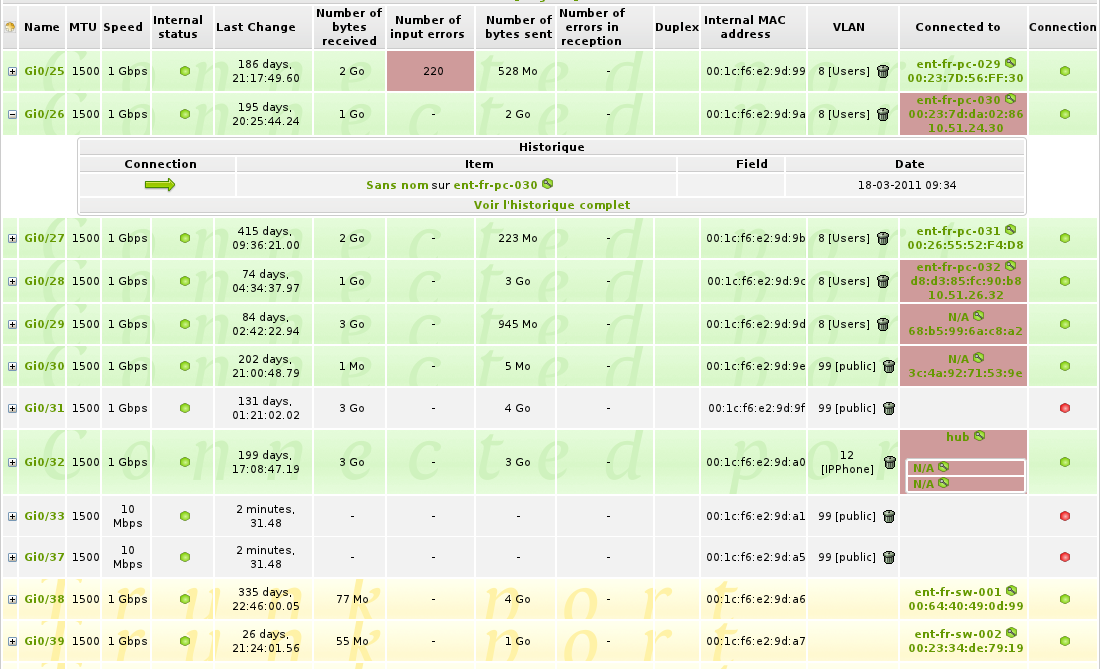
\includegraphics[width=11.7cm]{./pics/switch_ports.png}
    \end{center}
\end{frame}

\begin{frame}
    \frametitle{SNMP: Imprimante (1/2)}

    \begin{block}{Informations générales}
    \begin{itemize}
    \item Serial number
    \item Manufacturer
    \item Model
    \item Firmware
    \item Memory
    \item Mac address
    \item etc
    \end{itemize}
    \end{block}
\end{frame}

\begin{frame}
    \frametitle{SNMP: Imprimante (2/2)}

    \begin{block}{Informations avancées}
    \begin{itemize}
    \item Etats des cartouches
    \item Compteur de page
    \end{itemize}
    \end{block}
\end{frame}

\begin{frame}
    \frametitle{SNMP: exemple d'une imprimante}

    \begin{center}
    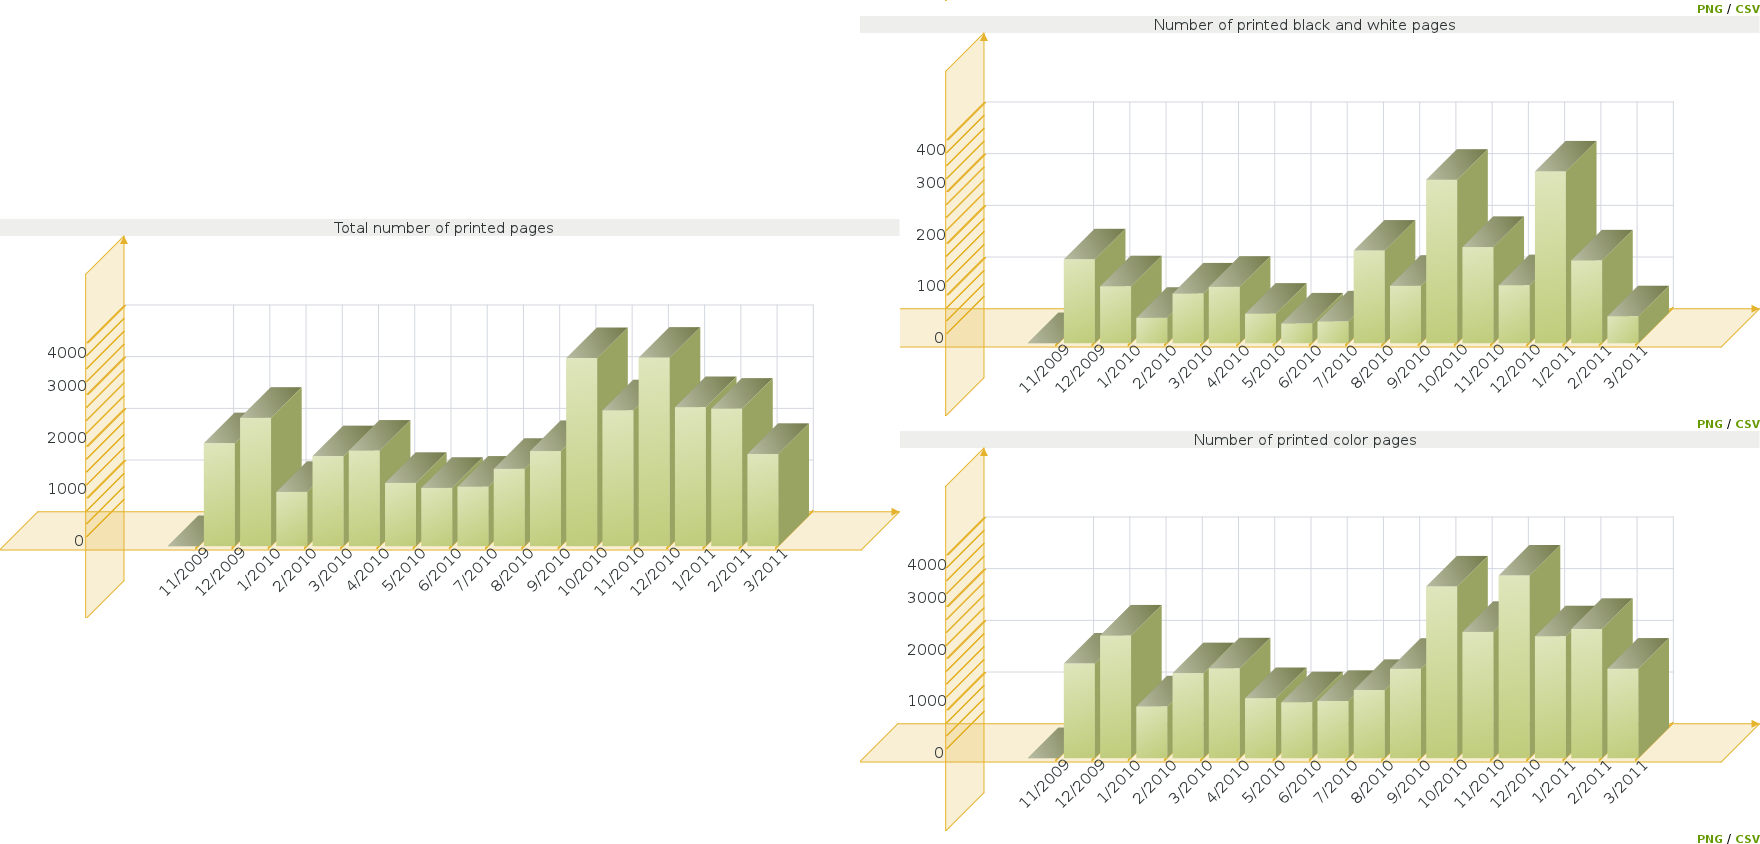
\includegraphics[width=11.7cm]{./pics/printer_graph.png}
    \end{center}
\end{frame}

\section{Tâche : Reveil sur le réseau}

\begin{frame}
    \frametitle{Wake On Lan}

    \begin{block}{WoL}
    \begin{itemize}
        \item Possiblité d'utiliser l'agent comme un proxy pour emettre des requêtes WoL.
    \end{itemize}
    \end{block}

\end{frame}

\begin{frame}
    \frametitle{Wake On Lan : Exemple}

    \begin{block}{Exemple}
    \begin{itemize}
    \item Un site distant
    \item 50 ordinateurs
    \end{itemize}
    \end{block}


    \begin{block}{Ce qu'on peut faire}
    \begin{itemize}
    \item Démarrer toutes les machines à 2h00 tout les soirs pour les mises à jour.
    \end{itemize}
    \end{block}

\end{frame}


\section{Tâche : La télédiffusion}

\begin{frame}
    \frametitle{La télédiffusion (1/2)}

    \begin{block}{Possibilité d'envoyer des actions a réaliser aux machines?}
    \begin{itemize}
        \item Pouvoir réaliser des actions sur les machines
        \item Envoyer des fichiers
        \item Réduire la bande passante grâce au “paire à paire”
    \end{itemize}
    Attention : ce n'est pas de la gestion de configuration.
    \end{block}

\WorkInProgress
\end{frame}

\begin{frame}
    \frametitle{La télédiffusion (2/2)}

    \begin{block}{Pourquoi un outil pour faire des télédiffusions vers les postes?}
    \begin{itemize}
        \item Utiliser l'interface existante de GLPI
        \item La gestion des droits de GLPI (groupes/profiles/entités)
    \end{itemize}
    \end{block}

\WorkInProgress
\end{frame}

\section{Tâche : vCenter/ESX/ESXi remote inventory}


\begin{frame}
    \frametitle{vCenter/ESX/ESXi}

    \begin{block}{Le problème}
    Des boites noire : On ne peut pas installer d'agent dessuss.
    \end{block}


\end{frame}

\begin{frame}
    \frametitle{vCenter/ESX/ESXi}

    \begin{block}{La solution}
    L'agent peut se connecter sur les équipements VMware via l'interface SOAP API:
        \begin{itemize}
                \item inventaire Hardware
                \item lister les Machines Virtuelles
                \item lister les ESX (dans les cas des ESX)
        \end{itemize}
    \end{block}

\end{frame}

\begin{frame}[fragile]
    \frametitle{vCenter/ESX/ESXi: en ligne de commande}

\begin{lstlisting}
fusioninventory-esx --host vcenter --user foo \ 
  --password bar --directory /tmp
\end{lstlisting}

Il ne reste plus qu'a pousser les inventaires :
\begin{lstlisting}
fusioninventory-injector -v --file /tmp/*.ocs \ 
  -u https://server/plugins/fusioninventory/
\end{lstlisting}

\end{frame}

\begin{frame}[fragile]
    \frametitle{vCenter/ESX/ESXi: l'interface GLPI}

 \begin{columns}
 \begin{column}[T]{4cm}
    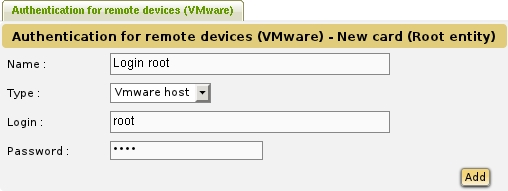
\includegraphics[height=4.0cm]{pics/esx-glpi.jpg}
 \end{column}
 \begin{column}[t]{6cm}
    \begin{block}{Une interface existe dans GLPI}
    \begin{itemize}
         \item Définir l'authentification
         \item Cibler un serveur vCenter/ESX/ESXi
         \item Planifier les inventaires
    \end{itemize}
    \end{block}
 \end{column}
\end{columns}




\end{frame}

\begin{frame}
\frametitle{ESX 1/2}


   \includegraphics[height=5cm]{./pics/esx1.png}
\end{frame}
%
\begin{frame}
\frametitle{ESX 2/2}


   \includegraphics[height=5cm]{./pics/esx2.png}
\end{frame}



\section{Tâche : L'inventaire}

\begin{frame}
    \begin{block}{Informations remontées (1/3)}
        \begin{itemize}
        \item BIOS
        \item modules PCI
        \item slots mémoires
        \item CPUs
        \item disques durs, lecteur, etc
        \item carte mère
        \item système d'exploitation
        \item écrans
        \item ports
        \item slots
        \item partitions
        \item logiciels
        \end{itemize}
    \end{block}
\end{frame}

\begin{frame}
    \begin{block}{Informations remontées (2/3)}
        \begin{itemize}
        \item utilisateurs connectés
        \item cartes vidéos
        \item machines virtuelles
        \item carte sons
        \item modems
        \item variables d'environnement
        \item équipements USB
        \item configuration réseau
        \item batteries
        \item imprimantes
        \item processus
        \item antivirus
        \item LVM
        \end{itemize}
        Android: carte SIM, IMEI , etc
    \end{block}
\end{frame}

\begin{frame}
    \begin{block}{Informations remontées (3/3)}
        Android: carte SIM, IMEI , etc
    \end{block}
\end{frame}

\section{La qualitaï!}

\begin{frame}
    \frametitle{Quelques métriques}

    \begin{block}{Aujourd'hui}
        \begin{itemize}
            \item 194 modules Perl
            \item 21851 lignes
            \item 938 tests unitaires
        \end{itemize}
    \end{block}

\end{frame}


\begin{frame}
    \frametitle{Quelques métriques}

    \begin{block}{Aujourd'hui}
        \begin{itemize}
            \item 194 modules Perl
            \item 21851 lignes
            \item \bf{938 tests unitaires} !
        \end{itemize}
    \end{block}

\end{frame}

\begin{frame}
    \frametitle{test-unitaire}

    \begin{block}{Comment ?}
        \begin{itemize}
            \item tester le parsing sur des OS qu'on a pas
            \item s'assurer que le code Win32 marche depuis un UNIX like \\
            \small{jusqu'a WMI et la base de registre}
            \item vérifier des choses pénibles \\
            \small{unicode, HTTPS, etc}
        \end{itemize}
    \end{block}

\end{frame}

\section{D'un point de vu développeur}

\begin{frame}
    \frametitle{Ce que FusionInventory peut apporter}

    \begin{block}{Plusieurs scénarii}
        \begin{itemize}
            \item Utiliser l'inventaire dans votre application
            \item Etendre la couverture de l'inventaire
            \item Interface avec GLPI ou autres \\
            \small{Uranos, bientôt OTRS, etc}
            \item Créer des nouvelles tâches
        \end{itemize}
    \end{block}

\end{frame}

\begin{frame}

    \begin{block}{Utiliser l'inventaire dans votre application}
    demo
    \end{block}

\end{frame}


\begin{frame}

    \begin{block}{Etendre la couverture de l'inventaire}
    demo
    \end{block}

\end{frame}

\begin{frame}

    \begin{block}{Créer des nouvelles tâches}
    Vous permet de récuperer facilement dans le bon contexte des objets :
    \begin{itemize}
      \item \$serveur
      \item \$config
      \item \$logger 
    \end{itemize}
    \end{block}

\end{frame}

\begin{frame}

    \begin{block}{Interface avec GLPI ou autres}
        \begin{itemize}
            \item SOAP (GLPI et OTRS)
        \end{itemize}
    \end{block}

\end{frame}

\section{La suite}

\begin{frame}
    \frametitle{What else?}

    \begin{center}
    \includegraphics[height=4.0cm]{pics/whatelse.jpg}
    \end{center}

\end{frame}

\begin{frame}
    \frametitle{Notre roadmap}

    Prochaines étapes :
    \begin{itemize}
        \item FusionInventory Agent 2.3.x
        \item \'{E}diteur de modèle SNMP XML
        \item Intégration avec nut 
    \end{itemize}

    Transition en cours :
    \begin{itemize}
        \item OCS/XML → REST/JSON
        \small{prévue pour l'agent 3.0.0\\utilisée par OTRS}
    \end{itemize}

\end{frame}


\section{Questions}

\begin{frame}
    \frametitle{Questions?}

%    \bf{Questions?}
    \begin{center}

    \includegraphics[height=5cm]{./pics/question.pdf}

    \end{center}
%    \includegraphics[height=7.5cm]{./pics/ask.jpg}

\end{frame}

\begin{frame}
    \frametitle{Thanks}

    \begin{block}{Thanks!}
        \begin{itemize}
            \item Windows \url{http://www.flickr.com/photos/aeu04117/430338509/sizes/z/in/photostream/}
            \item AIX \url{http://www.flickr.com/photos/pchow98/5115638572/}
            \item MacOSX \url{http://www.flickr.com/photos/adriannier/5555516312/sizes/l/in/photostream/}
            \item Cisco 6500 \url{http://www.flickr.com/photos/joachim\_s\_mueller/3084164647/sizes/z/in/photostream/}
            \item Teletubbies \url{http://www.flickr.com/photos/tudor/232849285/lightbox/}
            \item Worker \url{http://www.flickr.com/photos/wsdot/6783674428/sizes/l/in/photostream/}
            \item Bee \url{http://www.flickr.com/photos/8583446@N05/7454903214/sizes/l/in/photostream/}
            \item Montagne \url{http://www.flickr.com/photos/blmiers2/6167391543/sizes/l/in/photostream/} 
        \end{itemize}
    \end{block}
\end{frame}




\end{document}
